\documentclass[border=10pt]{standalone}
\usepackage{pgfplots}
\pgfplotsset{compat=1.18}
\begin{document}
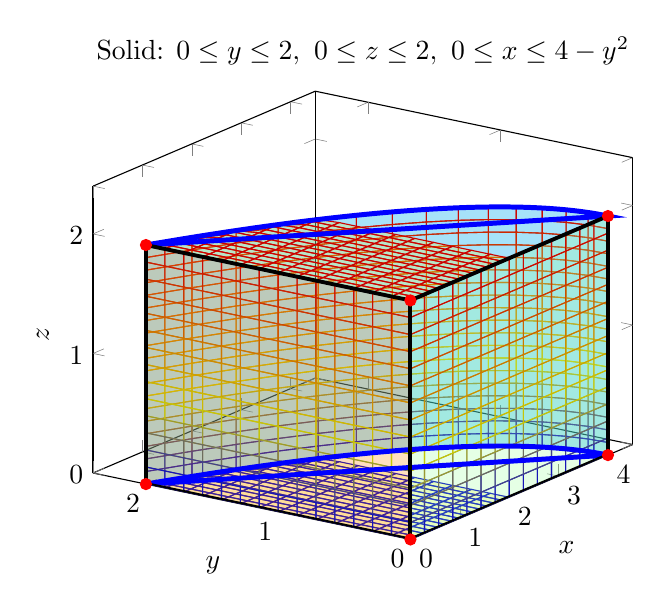
\begin{tikzpicture}
\begin{axis}[
    title={Solid: $0\le y\le 2,\ 0\le z\le 2,\ 0\le x\le 4-y^2$},
    xlabel={$x$}, ylabel={$y$}, zlabel={$z$},
    xmin=0, xmax=4.5, ymin=0, ymax=2.4, zmin=0, zmax=2.4,
    xtick={0,1,2,3,4}, ytick={0,1,2}, ztick={0,1,2},
    view={-55}{22},
    every axis plot/.append style={line width=0.4pt}
]

% Parabolic cylindrical surface
\addplot3[surf, samples=20, samples y=15,
          domain=0:2, y domain=0:2,
          variable=\s, variable y=\t,
          fill opacity=0.35, color=cyan]
    ( {4 - \t*\t}, {\t}, {\s} );

% Bottom face z=0, parabolic region
\addplot3[surf, samples=15, samples y=15,
          domain=0:2, y domain=0:2,
          variable=\s, variable y=\t,
          fill opacity=0.20, color=yellow]
    ( {max(0, min(\s, 4-\t*\t))}, {\t}, {0} );

% Top face z=2
\addplot3[surf, samples=15, samples y=15,
          domain=0:2, y domain=0:2,
          variable=\s, variable y=\t,
          fill opacity=0.20, color=yellow]
    ( {max(0, min(\s, 4-\t*\t))}, {\t}, {2} );

% Left face x=0 (square)
\addplot3[surf, samples=15, samples y=15,
          domain=0:2, y domain=0:2,
          variable=\s, variable y=\t,
          fill opacity=0.25, color=orange]
    ( {0}, {\s}, {\t} );

% Front face y=0 (rectangle 0<=x<=4, 0<=z<=2)
\addplot3[surf, samples=15, samples y=15,
          domain=0:4, y domain=0:2,
          variable=\s, variable y=\t,
          fill opacity=0.25, color=green!40]
    ( {\s}, {0}, {\t} );

% Boundary edges (note: variable=\t for parabolic edges)
\addplot3[domain=0:2, samples=80, blue, line width=1.8pt, variable=\t]
    ({4-\t*\t}, {\t}, 0);
\addplot3[domain=0:2, samples=80, blue, line width=1.8pt, variable=\t]
    ({4-\t*\t}, {\t}, 2);
\addplot3[black, line width=1.4pt] coordinates {(0,0,0) (4,0,0)};
\addplot3[black, line width=1.4pt] coordinates {(0,0,0) (0,2,0)};
\addplot3[black, line width=1.4pt] coordinates {(0,0,2) (4,0,2)};
\addplot3[black, line width=1.4pt] coordinates {(0,0,2) (0,2,2)};
\addplot3[black, line width=1.4pt] coordinates {(0,0,0) (0,0,2)};
\addplot3[black, line width=1.4pt] coordinates {(4,0,0) (4,0,2)};
\addplot3[black, line width=1.4pt] coordinates {(0,2,0) (0,2,2)};

% Vertices
\addplot3[only marks, mark=*, mark size=2pt, color=red]
    coordinates {(0,0,0) (4,0,0) (0,2,0) (0,0,2) (4,0,2) (0,2,2)};

\end{axis}
\end{tikzpicture}
\end{document}